\documentclass{article}
\usepackage{graphicx}

\title{Arrow’s Impossibility Theorem}
\author{Cecilia Sun}

%% \blurb{Say you’re Gru of <em>Despicable Me</em> fame, and you and your minions have just discovered a previously uninhabited island, on which you want to establish a new evil lab for you to conduct your evil experiments...}

\begin{document}

\maketitle
\begin{center}
    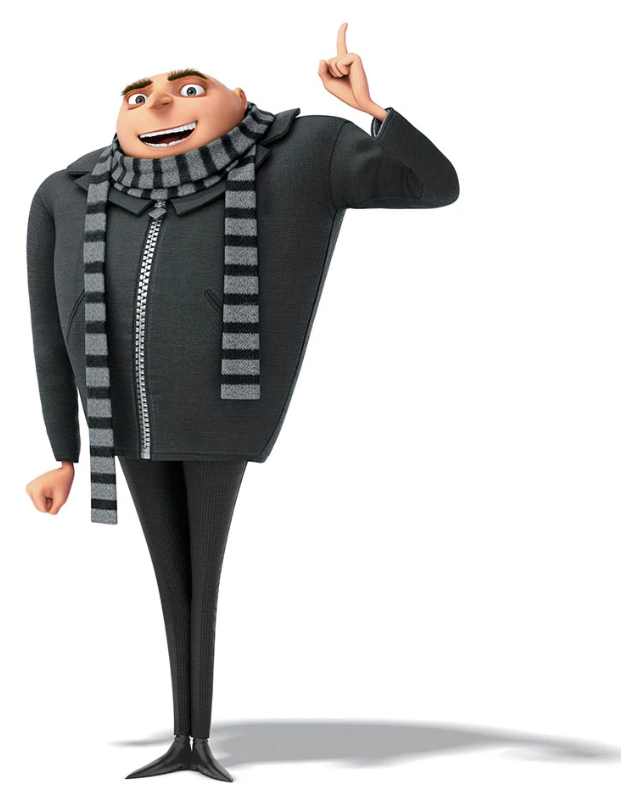
\includegraphics[scale=0.35]{images/gru.png}
\end{center}

Say you’re Gru of \textit{Despicable Me} fame, and you and your minions have just discovered a previously uninhabited island, on which you want to establish a new evil lab for you to conduct your evil experiments. Since you are Gru and must return home soon to be with Margo, Edith, and Agnes, your three adopted children, you have chosen a group of minions to stay on the island to do your evil bidding while you and the others return. However, the island minions soon run into an issue --- with you away from the island, who is going to be their leader? 

The minions suggest several voting schemes, and your job is to evaluate each of them and decide which one you want the minions to use:
\begin{itemize}
	\item \textbf{Stuart’s method}: Stuart is sensible, and proposes that each of the minions votes for one candidate. He will then count the number of votes each candidate has and use that to create a ranking of the candidates, and the minions will elect the candidate with the most votes.
	\item \textbf{Kevin’s method}: Kevin thinks the minions should take into account the second, third, etc. preferences of each individual minion. He proposes that they have each minion rank each of the $n$ candidates. For each ballot, the first choice candidate gets $n$ points, the second choice candidate gets $n-1$ points, etc. The candidates will be ranked based on their point total, and the minion with the greatest point total wins.
	\item \textbf{Bob’s method}: Bob is a dictator. Bob will rank all the candidates, and the minions will elect whoever Bob chooses as the winner. 
\end{itemize}

Ideally, want our voting systems to be \textit{fair} --- but what exactly does ``fair’’ mean? We might start with some criteria that will help us determine what a ``fair” system looks like:
\begin{itemize}
	\item \textbf{Universality}: We want our election system to be deterministic: in other words, there is no randomness involved in deciding who the winner is. Two identical sets of ballots should produce the same ranking and thus elect the same person every single time. 
	\item \textbf{Independence of irrelevant alternatives (IIA)}: The ranking between two candidates $x$ and $y$ should depend only on people’s preferences between $x$ and $y$; in other words, changes in individual voters’ preferences of any other candidate (say, $z$), should not impact the final ranking of $x$ and $y$ relative to each other. 
	For instance, if in the final ranking, Stuart is ranked higher than Kevin, then Stuart should be ranked higher than Kevin even if we disqualify Bob from the election. 
	
What happens when we don’t have IIA? Well, then there’s a potential for something like this to happen:
	%todo for cecilia: 
	%aroehus cropping is bad, i will fix later
	\begin{center}
	    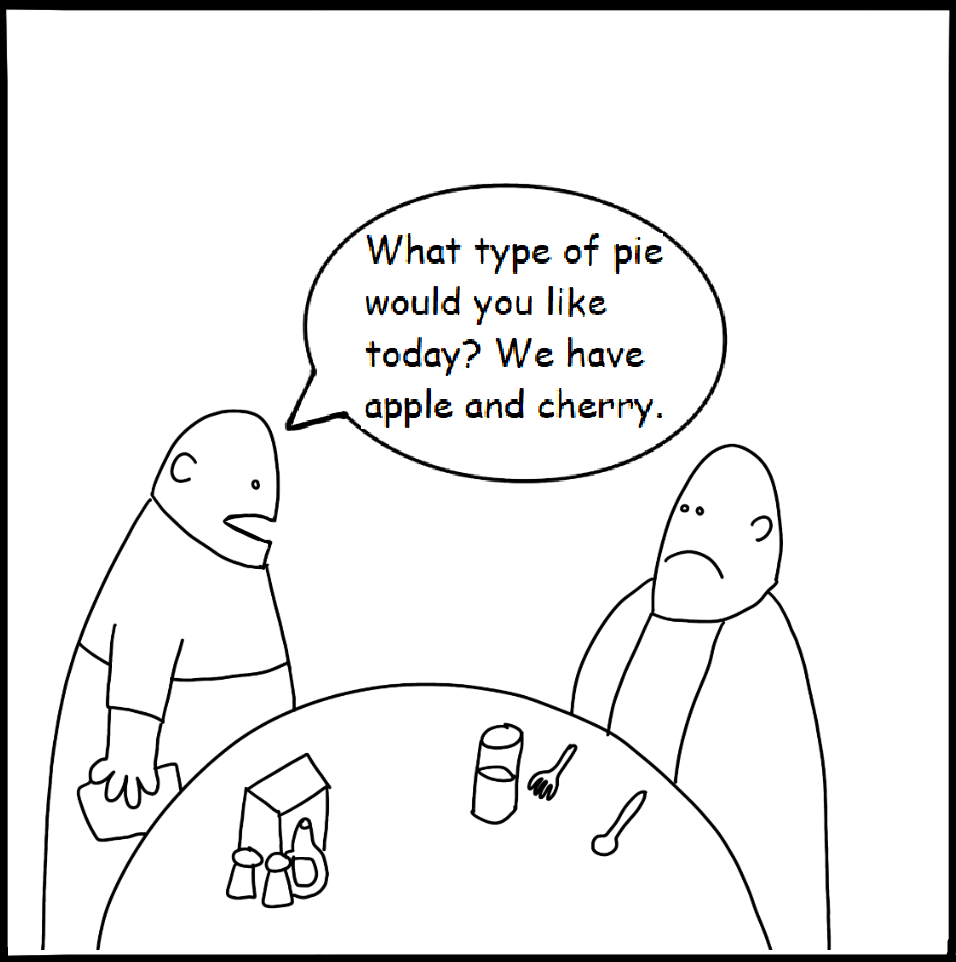
\includegraphics[width=\linewidth]{images/minions1.png}
	    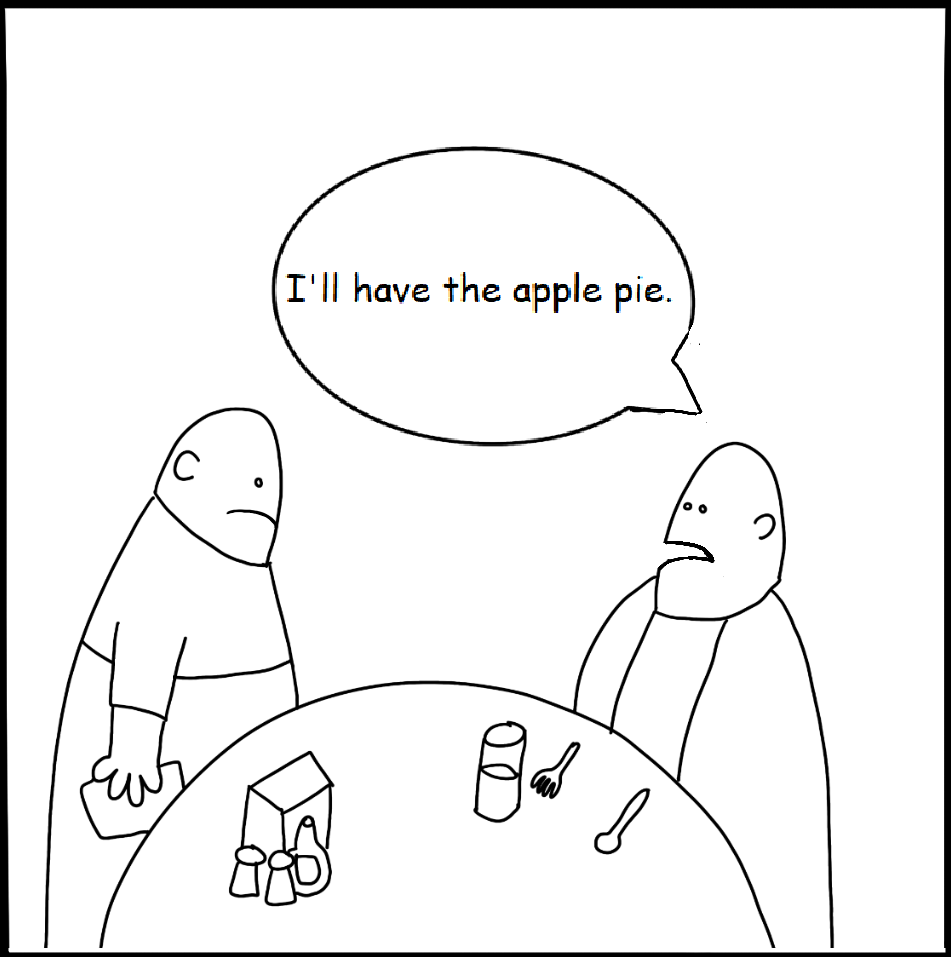
\includegraphics[width=\linewidth]{images/minions2.png}
	    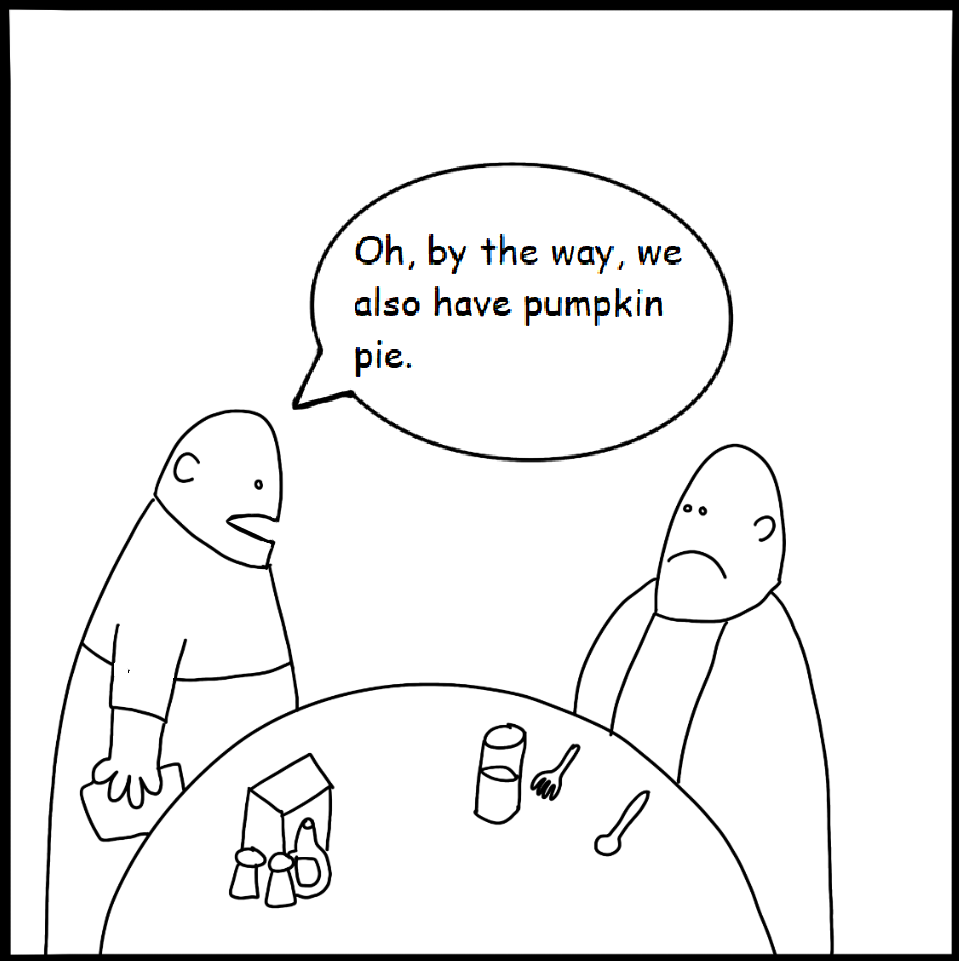
\includegraphics[width=\linewidth]{images/minions3.png}
	    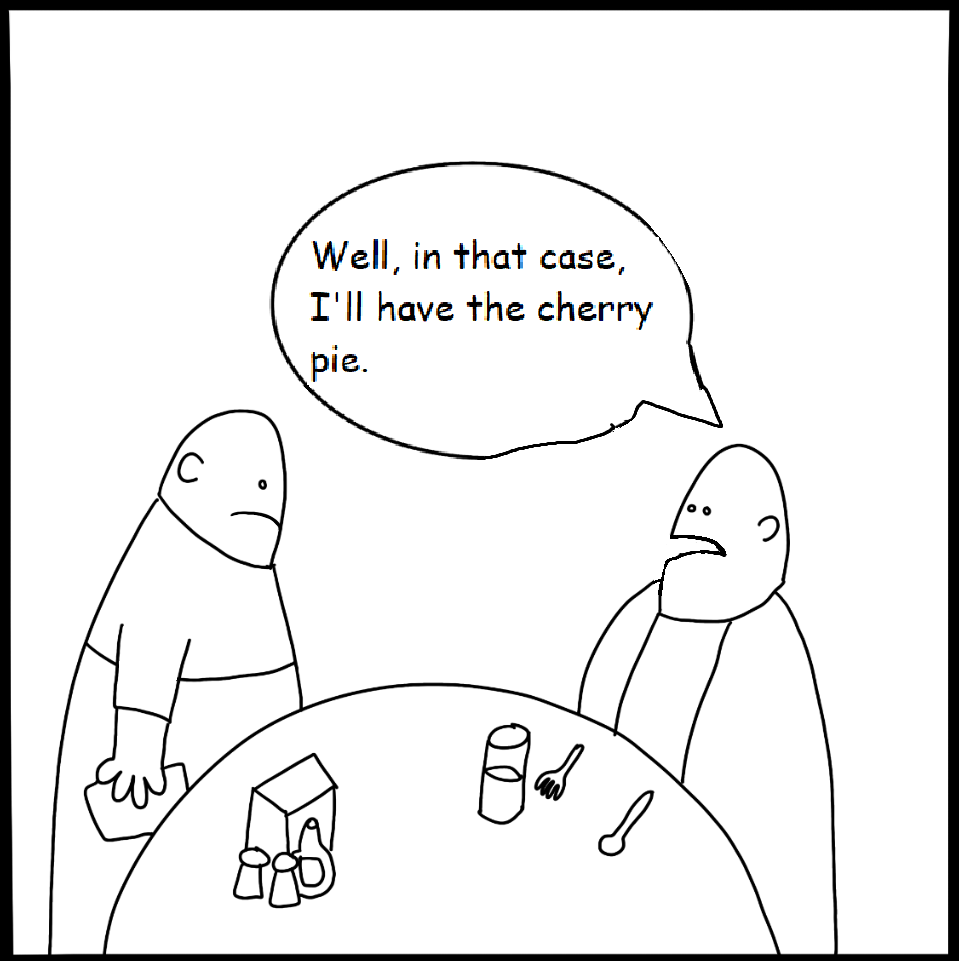
\includegraphics[width=\linewidth]{images/minions4.png}
	\end{center}
 
	\item \textbf{Monotonicity}: If an individual voter changes their vote by ranking one of the candidates higher, then the candidate’s position in the final ranking should either be higher or unchanged; in other words, a voter should not be able to hurt a candidate’s final ranking by ranking them higher. Similarly, a voter should not be able to boost a candidate’s final ranking by ranking them lower. 
	\item \textbf{Non-imposition}: It should be possible for any candidate to get elected! 
\end{itemize}

Let’s look at each of the three minions’ proposed strategies and evaluate their fairness based on our criteria:

\textbf{Stuart’s method}: Rank the candidates based on the number of first place votes they receive.
\begin{itemize}
	\item \textbf{Universality}: Stuart’s method \textbf{satisfies} universality: there is no randomness involved in his method.
	\item \textbf{IIA}: Stuart’s method \textbf{violates} IIA. Consider the following election between Stuart (S), Kevin (K), and Bob (B), where each column represents an individual voter’s ballot and the number of voters who had that ballot:
	\[
		\begin{array}{c|ccc}
				& 49 & 48 & 3 \\
			\text{1st} & S & K & B \\
			\text{2nd} & K & B & K \\
			\text{3rd} & B & S & S
		\end{array}
	\]

	Stuart wins this election, but if Bob is disqualified from the election, then the three votes for Bob will go to Kevin and he will then beat Stuart! 
	\item \textbf{Monotonicity}: Stuart’s method \textbf{satisfies} monotonicity: if a candidate has the most first-place votes, then giving them more first place votes will only put them higher in the ranking. 
	\item \textbf{Non-imposition}: Stuart method \textbf{satisfies} non-imposition: if all the minions rank a candidate first, then that candidate will win, and this is true of all candidates. 
\end{itemize}
Okay, so Stuart’s method is alright, but it does violate IIA, and in a pretty egregious fashion: in the example case, there are two candidates who are head to head and a third candidate who has very little support, which mimics a lot of real elections! 

\textbf{Kevin’s method}: For each ballot, give the first choice candidate $n$ points, the second choice gets $n-1$ points, etc. Then rank the candidates based on their point totals. 
\begin{itemize}
	\item \textbf{Universality}: Kevin’s method \textbf{satisfies} universality: there is no randomness involved in his method.
	\item \textbf{IIA}: Kevin’s method \textbf{violates} IIA. Consider the following election between Stuart (S), Kevin (K), Bob (B), and Dave (D):
	\[
		\begin{array}{c|ccc}
				& 14 & 8 & 4 \\
			\text{1st} & S & K & D \\
			\text{2nd} & K & D & S \\
			\text{3rd} & B & B & B \\
			\text{4th} & D & S & K
		\end{array}
	\]

	If we use Kevin’s method to determine the winner of this election, then Kevin wins with $78$ points. However, if we take Bob out of the election, then Stuart wins the election! 
	\item \textbf{Monotonicity}: Kevin’s method \textbf{satisfies} monotonicity: if a candidate has the most points, then ranking them higher will only increase their point count, and they can only move higher in the final ranking.
	\item \textbf{Non-imposition}: Kevin’s method \textbf{satisfies} non-imposition: if all the minions rank a candidate first, then that candidate will win, and this is true of all candidates. 
\end{itemize}
Even though Kevin’s method \textit{seems} to be more fair than Stuart's method, it still has the same IIA issues! 

\textbf{Bob’s method}: The ranking of candidates on Bob’s ballot is also the final ranking of candidates. 
\begin{itemize}
	\item \textbf{Universality}: Bob’s method \textbf{satisfies} universality: there is no randomness involved in his method.
	\item \textbf{IIA}: Bob’s method \textbf{satisfies} IIA! If a candidate drops out of the election, then the candidates’ placements relative to each other is the same since they are the same on Bob’s ballot, which is the only one that matters.
	\item \textbf{Monotonicity}: Bob’s method \textbf{satisfies} monotonicity. If a minion other than Bob changes their ballot, then all the candidates’ final placements remain the same, since Bob’s ballot is constant. If Bob changes his ballot to move a candidate higher, then the candidate will also be higher in the final ranking since the final ranking is determined by Bob’s ballot. 
	\item \textbf{Non-imposition}: Bob’s method \textbf{satisfies} non-imposition: if Bob ranks a candidate first, then that candidate wins, and this is true for all candidates
\end{itemize}

According to our criteria, Bob’s method is actually the fairest out of all the proposed methods! 

In 1950, economist Kenneth Arrow proved that, in fact, the only voting system that satisfies \textit{all} the fairness criteria is a dictatorship! 

This result may seem shocking, but its practicality has been questioned even by Arrow himself. Though there might exist extreme cases in which voting systems do things we don’t want them to do, if they, like Stuart and Kevin’s suggestions, are reasonable enough, then we can expect them to work enough of the time. ``Most systems are not going to work badly all of the time," said Arrow. ``All I proved is that all can work badly at times."
\end{document}
